\documentclass{beamer}
% Se usi XeLaTeX/LuaLaTeX non serve inputenc
\usepackage[utf8]{inputenc}
\usepackage{graphicx}
\usepackage{booktabs}
\usepackage{amsmath,amssymb}
\usepackage{microtype}

% Aggiungi path tema personalizzato
\makeatletter
\def\input@path{{theme/}}
\makeatother

% Tema accademico personalizzato
% Opzioni disponibili: legacy, dark, vibrant, icons, minimalblocks, academic
% Per stile più formale usiamo solo 'academic'; puoi aggiungere 'dark' se desideri modalità scura.
\usetheme[academic]{CleanEasy}
% (Modalità accademica attivata. Rimosso codice di debug e frame diagnostico.)

% --- Informazioni del Titolo ---
\title[Music Genre Classification]{Music Genre Classification: A Replication Study}
\author{Alessandro Potenza \and Camilla Sed}
\institute[Politecnico di Milano]{
    Politecnico di Milano \\
    Scuola di Ingegneria Industriale e dell'Informazione \\
    Laurea Magistrale in Computer Science and Engineering
}
\date{Academic Year 2024-2025}

% Compilazione consigliata: XeLaTeX o LuaLaTeX per font moderni
\begin{document}

% --- SLIDE 1: TITOLO ---
\begin{frame}
    \titlepage
\end{frame}

% --- SLIDE 2: INTRODUCTION & MOTIVATION ---
\begin{frame}
    \frametitle{Introduction: The Task}
    \begin{block}{What is Music Genre Classification (MGC)?}
        MGC is a fundamental task in Music Information Retrieval (MIR) that automatically categorizes music tracks into predefined genres based on their audio content.
    \end{block}
    \begin{columns}
        \begin{column}{0.5\textwidth}
            \textbf{Applications:}
            \begin{itemize}
                \item Music Recommendation
                \item Library Organization
                \item Content Discovery
            \end{itemize}
        \end{column}
        \begin{column}{0.5\textwidth}
            \textbf{The Reference Paper:}
            \begin{itemize}
                \item "Novel mathematical model..." by Patil et al. [3].
                \item Proposed a U-Net-like architecture.
                \item \textbf{Claimed a remarkable 99.41\% accuracy} on the GTZAN dataset.
            \end{itemize}
        \end{column}
    \end{columns}
\end{frame}

% --- SLIDE 3: PROJECT GOALS ---
\begin{frame}
    \frametitle{Our Project Goals}
    \begin{enumerate}
        \item \textbf{Replicate and Validate}: Implement the U-Net architecture and rigorously evaluate its performance on GTZAN to validate the paper's central claim.
        \vspace{1cm}
        \item \textbf{Compare and Analyze}: Compare this architecture against two other common CNN designs to understand its relative strengths.
        \vspace{1cm}
        \item \textbf{Extend and Generalize}: Assess the model's robustness by testing it on three additional, diverse datasets.
    \end{enumerate}
\end{frame}

% --- SLIDE 4: DATASETS ---
\begin{frame}
    \frametitle{The Datasets}
    A diverse set of datasets to test replication, complexity, and generalization.
    \begin{itemize}
        \item \textbf{GTZAN}: The primary dataset for our replication study. 1,000 tracks across 10 genres. The standard benchmark.
        \vspace{0.5cm}
        \item \textbf{FMA Small}: A more challenging and realistic benchmark. 8,000 tracks across 8 genres.
        \vspace{0.5cm}
        \item \textbf{Indian Music Genre (IMG)}: A non-Western dataset to test domain adaptation. 5 genres.
        \vspace{0.5cm}
        \item \textbf{Tabla Taala}: A specialized rhythmic dataset to test fine-grained pattern recognition. 8 rhythmic cycles.
    \end{itemize}
\end{frame}

% --- SLIDE 5: FEATURE EXTRACTION ---
\begin{frame}
    \frametitle{Feature Extraction: From Audio to Image}
    \begin{block}{Why Mel-Spectrograms?}
        We convert 1D audio signals into 2D image-like representations to leverage the power of CNNs. Mel-spectrograms are perceptually motivated and align with human hearing, making them an ideal feature for audio tasks.
    \end{block}
    This process involves:
    \begin{enumerate}
        \item Loading and Framing the audio signal.
        \item Applying a Short-Time Fourier Transform (STFT).
        \item Converting to the Mel scale.
        \item Applying Logarithmic Scaling (decibels).
    \end{enumerate}
\end{frame}

% --- SLIDE 6: MEL-SPECTROGRAM VISUALIZATION [IMMAGINE] ---
\begin{frame}[plain]
    \frametitle{Visualizing the Features: Waveform vs. Mel-Spectrogram}
    \begin{figure}
        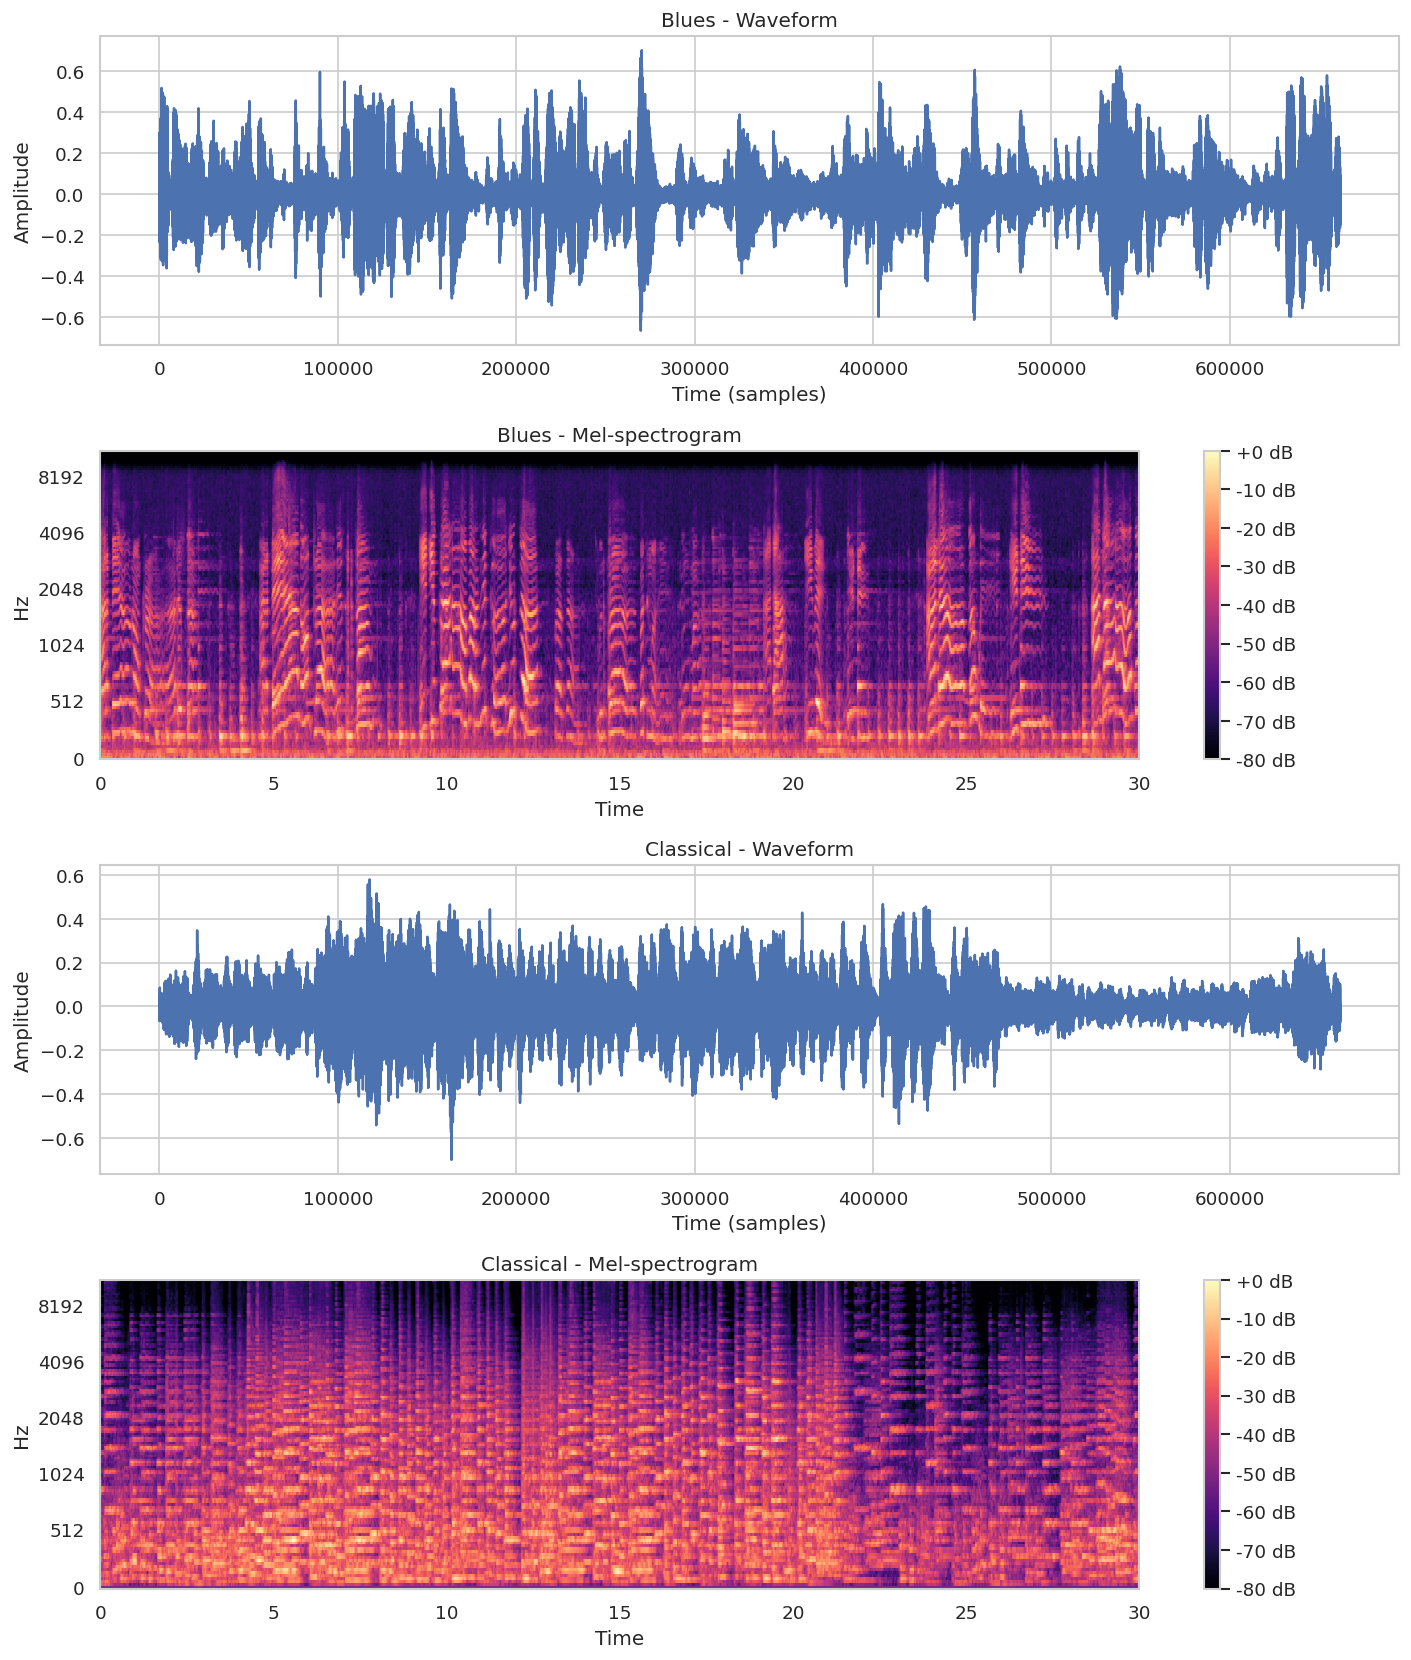
\includegraphics[width=\textwidth, height=0.7\textheight, keepaspectratio]{images/blues_waveform.png}
        \caption{Comparison for Blues (top) and Classical (bottom) tracks. The CNN learns to recognize these distinct visual textures.}
    \end{figure}
\end{frame}

% --- SLIDE 7: DATA PARTITIONING & LEAKAGE ---
\begin{frame}
    \frametitle{Data Partitioning and Slicing}
    \begin{block}{Slicing Strategy}
        Each 30-second track was sliced into 10 non-overlapping 3-second segments. This increases the training data tenfold (e.g., 600 training tracks $\rightarrow$ 6,000 samples).
    \end{block}

    \begin{alertblock}{Crucial Step: Avoiding Data Leakage}
        The dataset was split into train/validation/test sets (60/20/20) \textbf{at the track level, BEFORE slicing}. This is vital to prevent the model from "cheating" by recognizing a song's unique fingerprint across different sets.
    \end{alertblock}
\end{frame}

% --- SLIDE 8: MODEL ARCHITECTURES: THE COMPETITORS ---
\begin{frame}
    \frametitle{Model Architectures: The Competitors}
    We implemented three distinct CNNs for a comprehensive comparison.
    % Spazio sopra i blocchi numerati (prima era distribuito sotto i titoli)
    \vspace{0.9em}
    \begin{columns}
        \begin{column}{0.5\textwidth}
            \textbf{1. Efficient-VGG}
            \vspace{0.3em}% piccolo spazio solo sotto il titolo
            {\setlength{\itemsep}{5pt}\setlength{\topsep}{2pt}% local list spacing
            \begin{itemize}
                \item Lightweight baseline.
                \item Simple VGG structure + SE blocks.
                \item \textbf{~35k parameters}.
            \end{itemize}}
        \end{column}
        \begin{column}{0.5\textwidth}
            \textbf{2. ResSE-AudioCNN}
            \vspace{0.3em}
            {\setlength{\itemsep}{5pt}\setlength{\topsep}{2pt}
            \begin{itemize}
                \item Deeper, more powerful.
                \item Based on Residual Networks (ResNets) + SE blocks.
                \item \textbf{~1.23M parameters}.
            \end{itemize}}
        \end{column}
    \end{columns}
\end{frame}

% --- SLIDE 9: MODEL ARCHITECTURES: THE CHAMPION ---
\begin{frame}
    \frametitle{Model Architectures: The Champion (U-Net Classifier)}
    \begin{block}{Our Implementation of the Patil et al. Model}
        A U-Net-based architecture adapted for classification.
    \end{block}
    \begin{itemize}
        \item It uses only the \textbf{encoder (contracting) path} of a standard U-Net to learn hierarchical features at multiple resolutions.
        \item Three down-sampling blocks followed by a bottleneck.
        \item A \textbf{Global Average Pooling layer} and a Dense layer perform the classification.
        \item \textbf{~1.18M parameters}.
    \end{itemize}
\end{frame}

% --- SLIDE 10: TRAINING PROTOCOL ---
\begin{frame}
    \frametitle{Training Protocol}
    For a fair and reproducible comparison, all models were trained with a standardized protocol.
    \begin{itemize}
        \item \textbf{Optimizer}: Adam (initial lr = 1e-3).
        \item \textbf{Loss}: Categorical Cross-Entropy.
        \item \textbf{Epochs/Batch}: Up to 120 epochs, batch size of 48.
        \item \textbf{Callbacks}: EarlyStopping, ReduceLROnPlateau, ModelCheckpoint.
        \item \textbf{Reproducibility}: All random seeds were fixed to 42.
    \end{itemize}
    Let's see the key hyperparameters...
\end{frame}

% --- SLIDE 11: TRAINING HYPERPARAMETERS [TABELLA] ---
\begin{frame}[plain]
    \frametitle{Key Training Hyperparameters}
    % --- Da inserire nel preambolo: \usepackage{booktabs} ---

\begin{table}
\centering
\caption{Key training hyperparameters used across experiments.}
\begin{tabular}{ll}
\toprule
\textbf{Hyperparameter} & \textbf{Value} \\
\midrule
Optimizer & Adam (initial lr = $1 \times 10^{-3}$) \\
Batch size (single-split) & 48 \\
Batch size (5-fold CV) & 16 \\
Epochs (max) & 120 (single-split), 60 (CV) \\
EarlyStopping patience & 25 (single-split), 10 (CV) \\
ReduceLROnPlateau factor & 0.2 \\
Mixed precision & enabled (\texttt{mixed\_float16}) \\
Random seeds & Python/NumPy/TensorFlow = 42 \\
\bottomrule
\end{tabular}
\end{table}
\end{frame}

% --- SLIDE 12: GTZAN RESULTS: OVERVIEW ---
\begin{frame}
    \frametitle{GTZAN Results: Performance \& Efficiency}
    \begin{block}{U-Net Audio Classifier is the Winner}
        It achieves the best balance of accuracy and computational efficiency among the tested models.
    \end{block}
    Here's a summary of the performance on the GTZAN test set.
\end{frame}

% --- SLIDE 13: GTZAN PERFORMANCE METRICS [TABELLA] ---
\begin{frame}[plain]
    \frametitle{Performance and Efficiency Metrics (GTZAN Test Set)}
    % --- Da inserire nel preambolo: \usepackage{booktabs} ---

\begin{table}
\centering
\caption{Performance and efficiency metrics on the GTZAN test set.}
\begin{tabular}{lccc}
\toprule
\textbf{Model} & \textbf{Test Accuracy} & \textbf{Parameters} & \textbf{Latency (ms)} \\
\midrule
UNet\_Audio\_Classifier & 0.823 & 1.18 M & 23.07 \\
ResSE\_Audio\_CNN & 0.798 & 1.23 M & 26.75 \\
Efficient\_VGG & 0.752 & 0.03 M & 14.77 \\
\bottomrule
\end{tabular}
\end{table}
\end{frame}

% --- SLIDE 14: GTZAN ACCURACY VS EFFICIENCY [IMMAGINE] ---
\begin{frame}[plain]
    \frametitle{Accuracy vs. Efficiency Trade-off}
    \begin{figure}
        \centering
        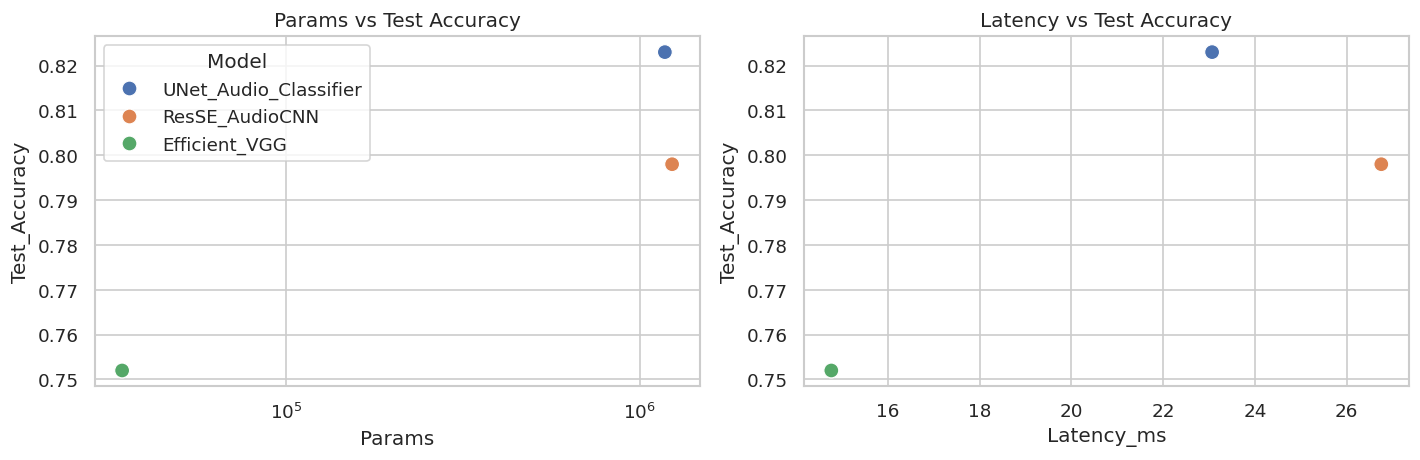
\includegraphics[width=\textwidth]{images/efficiency_accuracy.png}
        \caption{The U-Net model (blue) offers the best accuracy-efficiency trade-off compared to the comparable ResNet-based model (orange).}
    \end{figure}
\end{frame}

% --- SLIDE 15: ABLATION STUDY: SPECAUGMENT ---
\begin{frame}
    \frametitle{Ablation Study: The Impact of SpecAugment}
    \begin{block}{What is SpecAugment?}
        A data augmentation technique that randomly masks frequency bands and time steps in the spectrogram, forcing the model to learn more robust features.
    \end{block}
    \textbf{Question}: Does it always help?
    \textbf{Finding}: Only the U-Net architecture, our largest model, benefited. This suggests model capacity is crucial for leveraging this type of regularization. Simpler models may treat it as noise.
\end{frame}

% --- SLIDE 16: SPECAUGMENT RESULTS [IMMAGINE] ---
\begin{frame}[plain]
    \frametitle{Impact of SpecAugment on Test Accuracy}
    \begin{figure}
        \centering
        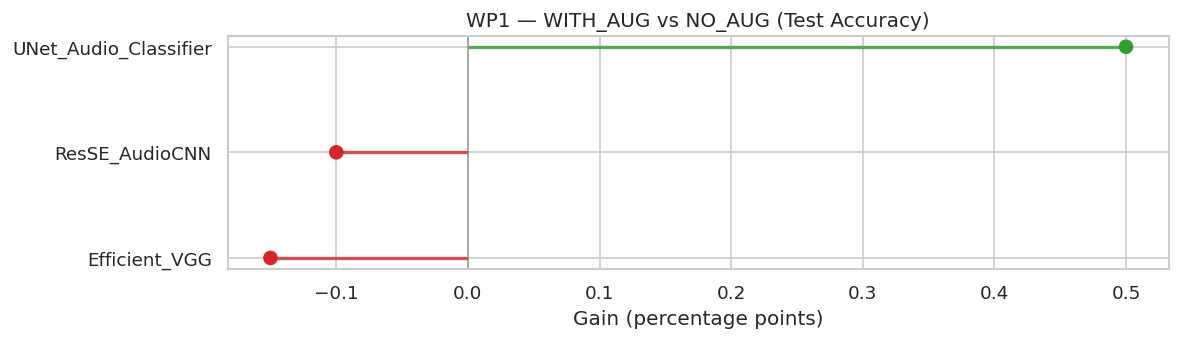
\includegraphics[width=0.95\textwidth]{images/with_without_aug.png}
        \caption{Change in test accuracy. Only the U-Net shows a positive gain.}
    \end{figure}
\end{frame}

% --- SLIDE 17: ROBUSTNESS CHECK: 5-FOLD CV ---
\begin{frame}
    \frametitle{Robustness Check: 5-Fold Cross-Validation}
    A single train/test split can be misleading. We performed a 5-fold cross-validation on the champion U-Net model for a more reliable performance estimate.

    \begin{alertblock}{Our Most Reliable Result on GTZAN}
        \centering
        \huge{90.44\%}
        \vspace{0.2cm}
        \Large{Mean Validation Accuracy}
    \end{alertblock}

    This result is substantially higher than our single-split accuracy (82.3\%) and has a very low standard deviation (0.68\%), demonstrating the model's stability.
\end{frame}

% --- SLIDE 18: WINNER MODEL ANALYSIS ---
\begin{frame}
    \frametitle{Analysis of the Winner Model's Performance}
    Where does the model succeed and fail?
    \begin{itemize}
        \item The model excels on genres with distinct acoustic signatures.
        \item Its primary weakness lies with genres that are spectrally similar.
    \end{itemize}
    Let's look at the per-class metrics.
\end{frame}

% --- SLIDE 19: CLASSIFICATION REPORT [TABELLA] ---
\begin{frame}[plain]
    \frametitle{Per-Class Classification Report (U-Net on GTZAN)}
    % --- Da inserire nel preambolo: \usepackage{booktabs} ---

\begin{table}
\centering
\caption{Per-class classification report for the U-Net model on GTZAN.}
\small % Puoi cambiare a \footnotesize se non entra
\begin{tabular}{lcccc}
\toprule
\textbf{Genre} & \textbf{Precision} & \textbf{Recall} & \textbf{F1-Score} & \textbf{Support} \\
\midrule
blues & 0.87 & 0.84 & 0.85 & 200 \\
classical & 0.96 & 1.00 & 0.98 & 200 \\
country & 0.75 & 0.80 & 0.78 & 200 \\
disco & 0.78 & 0.80 & 0.79 & 200 \\
hiphop & 0.77 & 0.74 & 0.76 & 200 \\
jazz & 0.89 & 0.96 & 0.93 & 200 \\
metal & 0.88 & 0.94 & 0.91 & 200 \\
pop & 0.76 & 0.89 & 0.82 & 200 \\
reggae & 0.91 & 0.69 & 0.79 & 200 \\
rock & 0.66 & 0.57 & 0.61 & 200 \\
\midrule
\textbf{Accuracy} & & & \textbf{0.82} & \textbf{2000} \\
\textbf{Macro Avg} & \textbf{0.82} & \textbf{0.82} & \textbf{0.82} & \textbf{2000} \\
\textbf{Weighted Avg} & \textbf{0.82} & \textbf{0.82} & \textbf{0.82} & \textbf{2000} \\
\bottomrule
\end{tabular}
\end{table}
\end{frame}

% --- SLIDE 20: GTZAN CONFUSION MATRIX [IMMAGINE] ---
\begin{frame}[plain]
    \frametitle{GTZAN Confusion Matrix: Visualizing the Errors}
    \begin{figure}
        \centering
        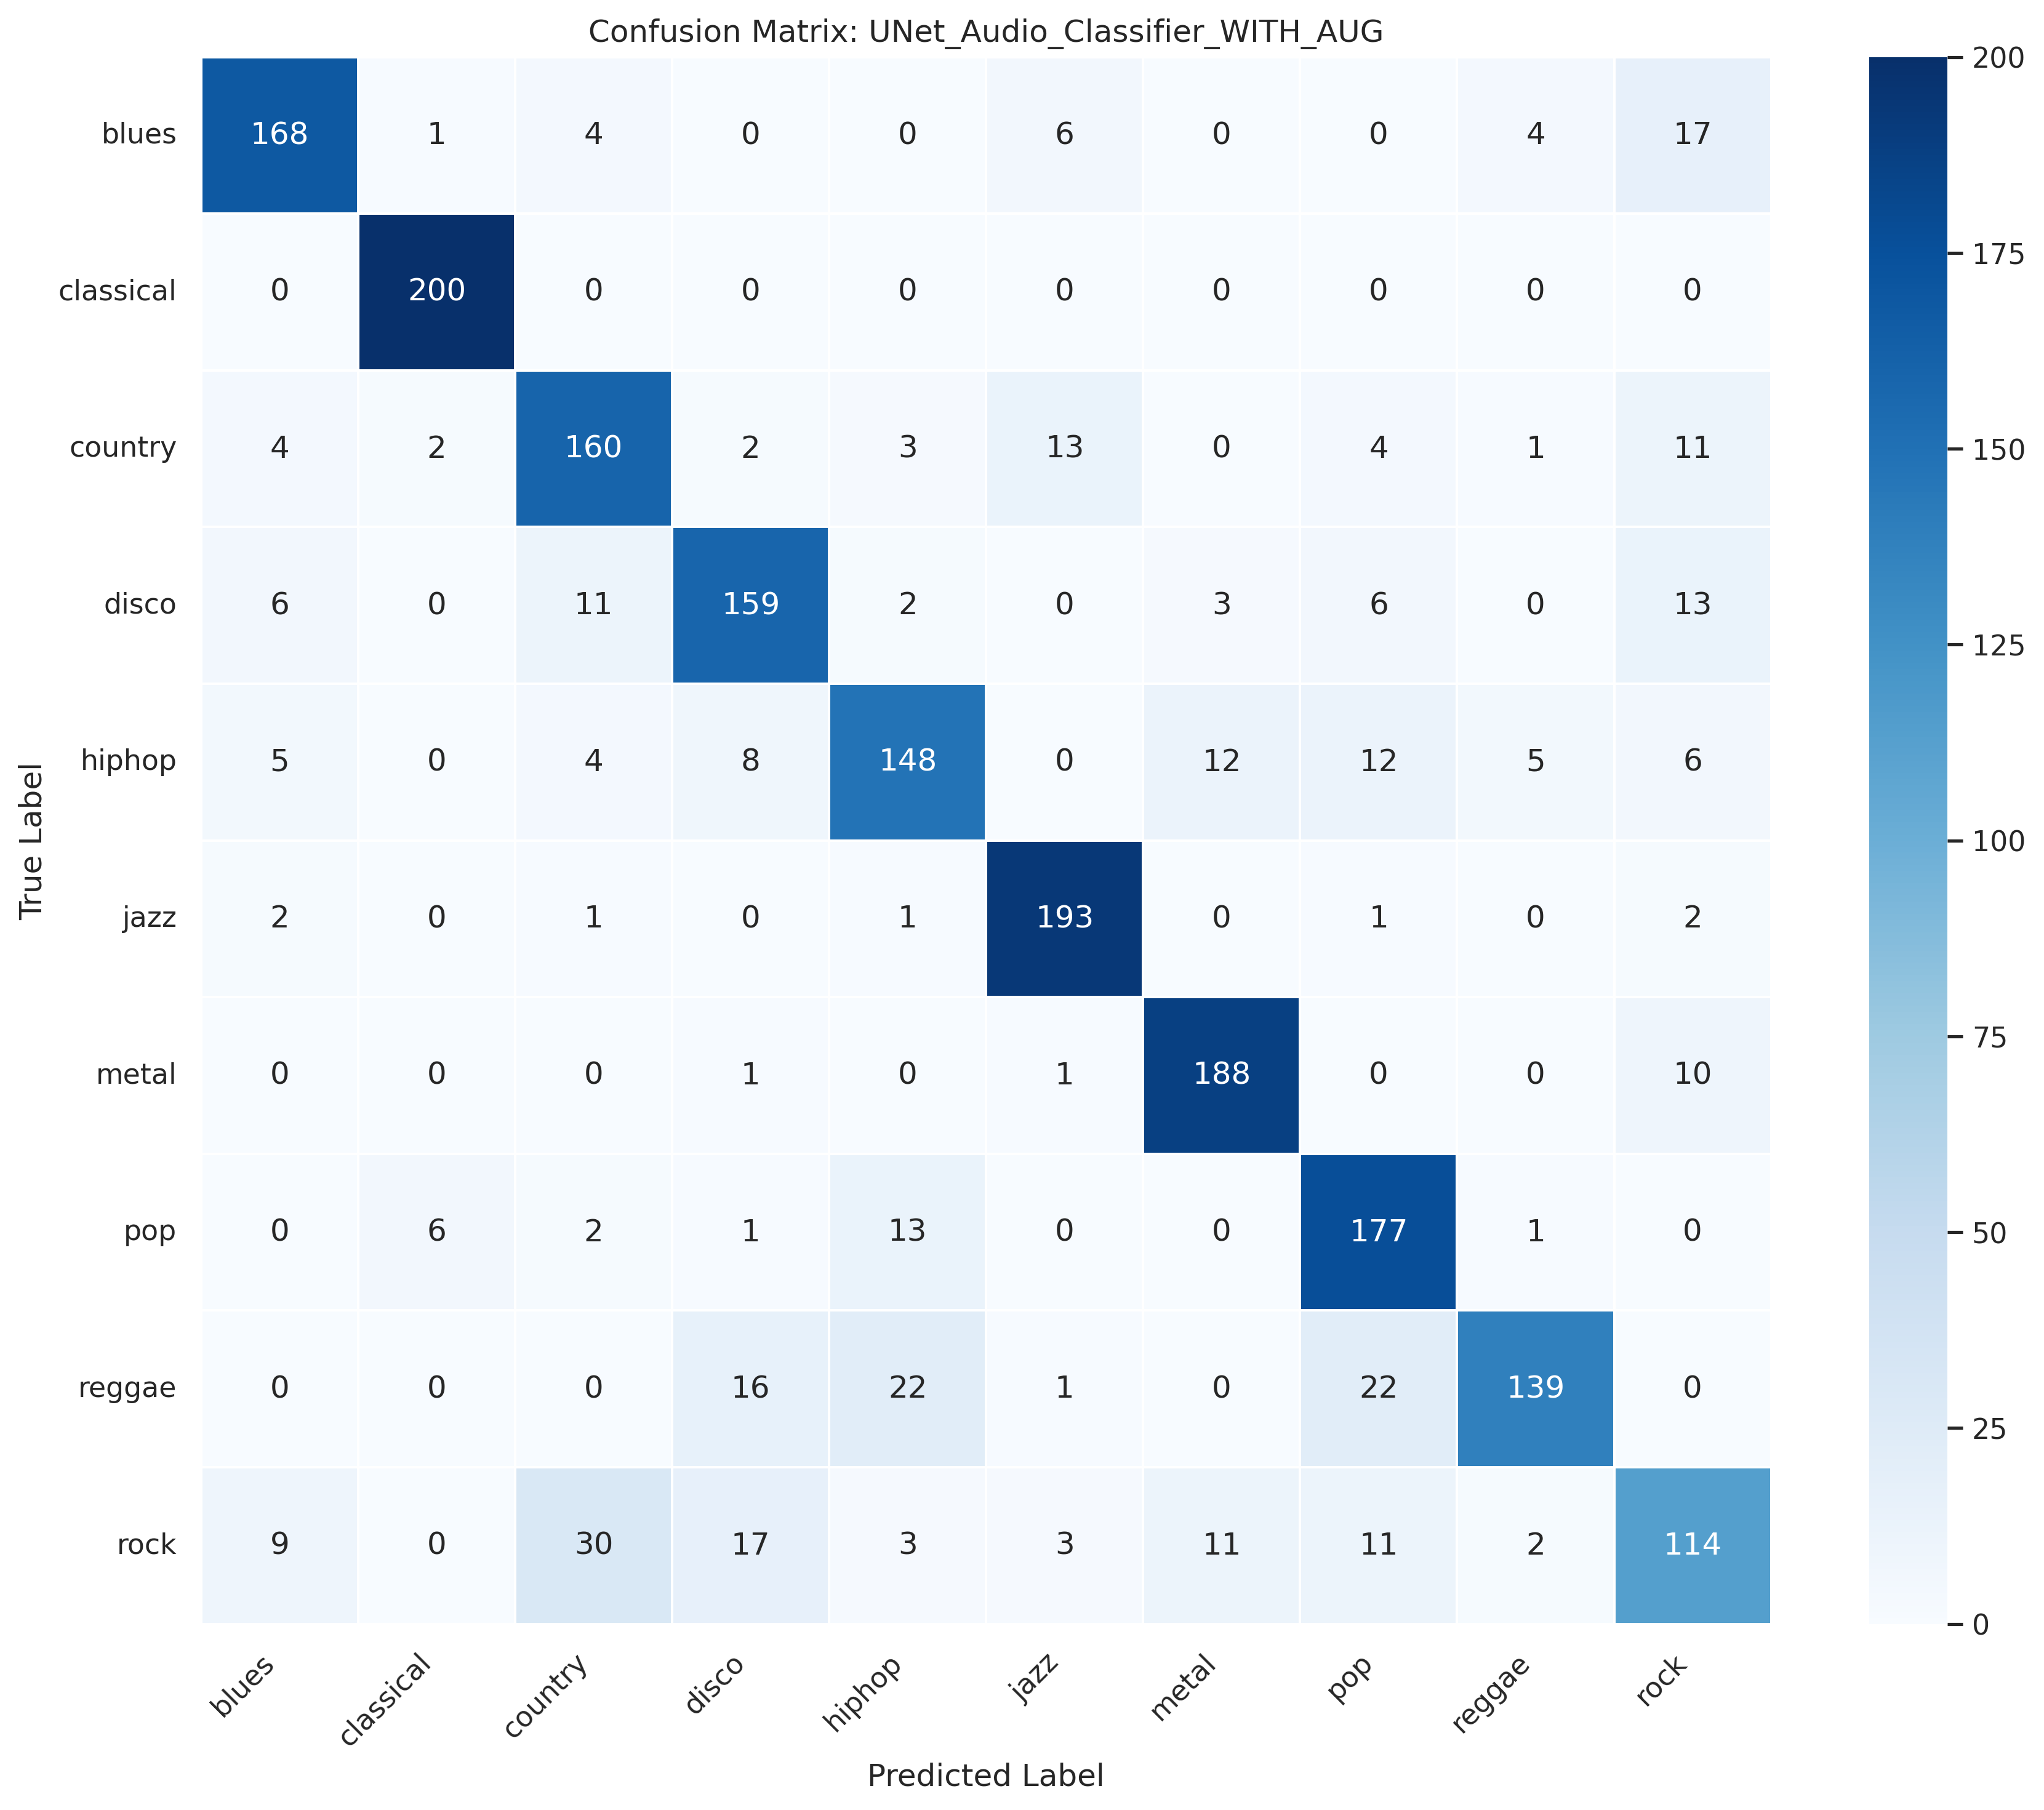
\includegraphics[width=\textwidth, height=0.8\textheight, keepaspectratio]{images/gtzan_cm.png}
    \end{figure}
\end{frame}

% --- SLIDE 21: CONFUSION MATRIX ANALYSIS ---
\begin{frame}
    \frametitle{Analysis of the Confusion Matrix}
    The confusion matrix confirms our findings:
    \begin{itemize}
        \item A strong diagonal indicates high overall accuracy.
        \item The low recall for 'rock' is explained by its confusion with spectrally similar genres like 'country' and 'disco'.
        \item Similarly, 'reggae' is often confused with 'hiphop'.
        \item These errors are musically coherent, highlighting the intrinsic difficulty of the task based on short 3-second clips.
    \end{itemize}
\end{frame}

% --- SLIDE 22: BEYOND GTZAN: CROSS-DATASET GENERALIZATION ---
\begin{frame}
    \frametitle{Beyond GTZAN: Cross-Dataset Generalization}
    We tested our champion U-Net model on three new datasets to assess its true capabilities.
    \begin{columns}
        \begin{column}{0.5\textwidth}
            \textbf{Strategy 1: From Scratch}
            \begin{itemize}
                \item \textbf{Dataset}: FMA Small
                \item \textbf{Challenge}: High complexity and realism.
            \end{itemize}
        \end{column}
        \begin{column}{0.5\textwidth}
            \textbf{Strategy 2: Transfer Learning}
            \begin{itemize}
                \item \textbf{Datasets}: Indian Music \& Tabla Taala
                \item \textbf{Challenge}: Domain shift (cultural and task-specific).
            \end{itemize}
        \end{column}
    \end{columns}
\end{frame}

% --- SLIDE 23: GENERALIZATION RESULTS [IMMAGINE] ---
\begin{frame}[plain]
    \frametitle{Performance Across All Datasets}
    \begin{figure}
        \centering
        
\includegraphics[width=\textwidth]{images/dataset_comparison.png}
        \caption{The success of transfer learning on Indian and Tabla datasets is evident when contrasted with the from-scratch training on FMA.}
    \end{figure}
\end{frame}

% --- SLIDE 24: GENERALIZATION RESULTS ANALYSIS ---
\begin{frame}
    \frametitle{Generalization Results: A Tale of Two Strategies}
    \begin{block}{Transfer Learning is Highly Effective}
        Features learned on Western music (GTZAN) can be successfully adapted to new domains.
    \end{block}
    \begin{itemize}
        \item \textbf{FMA Small (from scratch)}: 41.1\% accuracy. Much better than random (12.5\%), but shows the dataset's difficulty.
        \item \textbf{Indian Music (transfer)}: 72.2\% accuracy. Strong result, confirming feature universality.
        \item \textbf{Tabla Taala (transfer)}: \textbf{96.5\% accuracy}. Exceptional result, showing the model learned to recognize fine-grained rhythmic patterns.
    \end{itemize}
\end{frame}

% --- SLIDE 25: CROSS-DATASET CONFUSION MATRICES [IMMAGINE] ---
\begin{frame}[plain]
    \frametitle{Visualizing Generalization Performance}
    \begin{figure}
        \centering
        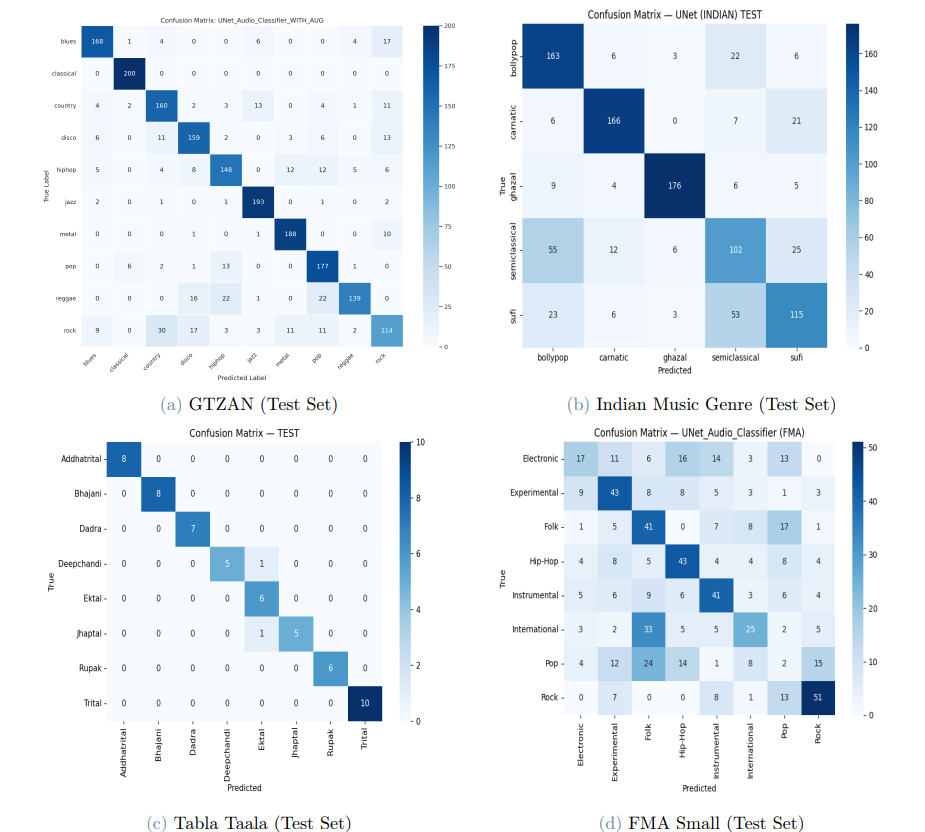
\includegraphics[width=\textwidth, height=0.7\textheight, keepaspectratio]{images/cms.png}
        \caption{Strong diagonals for GTZAN and Tabla Taala vs. a diffuse matrix for FMA Small, reflecting dataset complexity.}
    \end{figure}
\end{frame}

% --- SLIDE 26: DISCUSSION: THE PERFORMANCE DISCREPANCY ---
\begin{frame}
    \frametitle{Discussion: The Big Question}
    Why is there such a large gap between our results and the reference paper?

    \begin{columns}
        \begin{column}{0.5\textwidth}
            \begin{beamercolorbox}[sep=1em,center]{block title}
                \textbf{Patil et al. [3]}
            \end{beamercolorbox}
            \begin{beamercolorbox}[sep=1em,center]{block body}
                \Huge{99.41\%}
            \end{beamercolorbox}
        \end{column}
        \begin{column}{0.5\textwidth}
            \begin{beamercolorbox}[sep=1em,center]{block title alerted}
                \textbf{Our Best Result (5-Fold CV)}
            \end{beamercolorbox}
            \begin{beamercolorbox}[sep=1em,center,wd=\textwidth]{block body alerted}
                \Huge{90.44\%}
            \end{beamercolorbox}
        \end{column}
    \end{columns}
    
    A difference of \textbf{$\sim$9 percentage points} is too significant to be caused by minor architectural variations.
\end{frame}

% --- SLIDE 27: POTENTIAL SOURCES OF DISCREPANCY ---
\begin{frame}
    \frametitle{Potential Sources of Discrepancy}
    Our analysis points to methodological factors, not architectural ones.
    \begin{enumerate}
        \item \textbf{Data Splitting and Information Leakage (Leading Hypothesis)}:
        \begin{itemize}
            \item The original paper does not specify its splitting protocol.
            \item Randomly splitting \textit{after} slicing audio tracks is a common pitfall that transforms the task into \textit{audio fingerprinting}, leading to inflated scores.
            \item Our strict track-level split provides a more realistic evaluation.
        \end{itemize}
        \vspace{0.3cm}
        \item \textbf{Methodological Ambiguity}: The paper's "novel mathematical model" lacks specific details for perfect replication.
        \vspace{0.3cm}
        \item \textbf{Context of State-of-the-Art on GTZAN}: Accuracies of 90-95\% are typical. A near-perfect score of 99.41\% is a significant outlier.
    \end{enumerate}
\end{frame}

% --- SLIDE 28: CORROBORATION OF MODEL EFFICIENCY ---
\begin{frame}
    \frametitle{Corroboration of Model Efficiency}
    \begin{block}{One thing we can confirm...}
        Despite the accuracy discrepancy, our efficiency analysis validates a central premise of the paper.
    \end{block}
    
    Our experiments confirm that the U-Net based classifier provides a \textbf{superior balance of performance and computational cost} compared to a standard ResNet-based architecture.
    
    \begin{itemize}
        \item \textbf{UNet\_Audio\_Classifier}: 82.3\% accuracy, 1.18M params, 23.07 ms latency.
        \item \textbf{ResSE-AudioCNN}: 79.8\% accuracy, 1.23M params, 26.75 ms latency.
    \end{itemize}
    
    The U-Net's multi-scale encoder design is an effective choice for this task.
\end{frame}

% --- SLIDE 29: CONCLUSION & KEY FINDINGS ---
\begin{frame}
    \frametitle{Conclusion \& Key Findings}
    \begin{itemize}
        \item \textbf{U-Net Encoder is Effective}: We corroborate the architectural premise. Our champion model achieved a robust \textbf{90.44\%} accuracy on GTZAN, establishing a new, transparent, and reproducible benchmark.
        \vspace{0.4cm}
        \item \textbf{Performance Gap is Methodological}: The 99.41\% claim is an outlier, likely attributable to data leakage from an improper splitting protocol, not a superior architecture.
        \vspace{0.4cm}
        \item \textbf{Adaptability Through Transfer Learning}: The architecture shows excellent adaptability, achieving 96.5\% accuracy on the specialized Tabla Taala dataset.
        \vspace{0.4cm}
        \item \textbf{Importance of Rigor}: This work serves as a case study on the paramount importance of methodological transparency and robust validation in machine learning.
    \end{itemize}
\end{frame}

% % --- SLIDE 30: QUESTIONS ---
% \begin{frame}
%     \frametitle{Thank You}
%     \begin{center}
%         \Huge{\textbf{Questions?}}
%     \end{center}
% \end{frame}

\end{document}